%==========================================================================
% BEGIN SUGESTÕES PARA ESCRITA DO RELATÓRIO
%==========================================================================

\chapter{Sugestões para Escrita do Relatório}

    \section{Sugestões Gerais}
        <<O presente documento deverá servir de base para a escrita do relatório do trabalho realizado.>>

        <<O tipo de letra a utilizar deverá ser Arial.. Porém recomenda-se em situações de escrita de excertos de programas a utilização do tipo de letra Courier New.>>

        << Alguns estilos documento: Heading1, Heading2, Heading3, Normal e Footnote Text; foram especialmente modificados para os relatórios da presente disciplina.>>

        <<Os formatos e estilos de letra não devem estar constantemente a ser modificados ao longo do relatório. Tal situação dará origem a um relatório com um formato e apresentação muito heterogénea e com um aspecto pouco consistente.>>
    \section{Termos Estrangeiros}
        <<Os termos estrangeiros utilizados deverão ser apresentados num formato diferente do resto do texto, por exemplo: Data Warehouse (em itálico) ou "Data Warehouses" (entre aspas), devendo ser evitados sempre que se conheça uma tradução correcta para português. Para validação desses termos existem vários dicionários no mercado que poderão ser úteis.>>
    \section{Tabelas e Figuras}
        <<Caso seja necessário introduzir figuras ou tabelas no corpo do documento, estas devem seguir os formatos que se apresentam de seguida. Qualquer figura ou tabela deverá ter uma legenda associada, devendo esta estar correctamente apresentada no índice respectivo no início do relatório.>>
        

         \begin{figure}[!h]
            \centering
            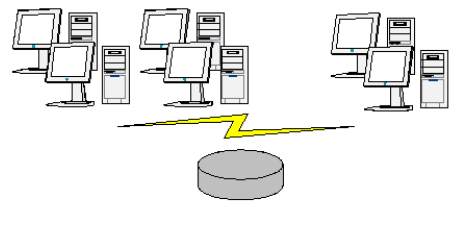
\includegraphics[scale=0.7]{images/example.png}
            \caption{Ilustração de inserção de uma figura e legenda.}
         \end{figure}
        
        \vspace*{0.2cm}
        
        \begin{table}[!h]
            \centering
            \begin{tabular}{|p{2cm}|p{2cm}|p{2cm}|p{2cm}|p{2cm}|}
               \hline
               \rowcolor{gray!20!white}
                Coluna1 & Coluna2 & Coluna3 & & ColunaN \\
                \hline
                        &         &         & &         \\
                \hline
                        &         &         & &         \\
                \hline
                        &         &         & &         \\
                \hline
                        &         &         & &         \\
                \hline
                        &         &         & &         \\
                \hline
            \end{tabular}
            \caption{Ilustração de inserção de uma tabela e sua legenda.}
        \end{table}
        
        
    \section{Siglas e Acrónimos}
        <<A utilização de siglas ou acrónimos deverão, tal como os termos estrangeiros, ser feita com base no seguinte formato: Bases de Dados (BD). Todas as siglas e acrónimos deverão ser apresentadas numa secção própria, no início (a seguir aos índices) ou no final (a seguir ao capítulo das conclusões e trabalho futuro) do relatório.
    \section{Referências Bibliográficas}
        <<A forma de apresentação das referências bibliográficas deverão estar de acordo com as regras definidas pela IEEE. Consultar www.ieee.org>>
    \section{Tipo de Ficheiro}
        <<O relatório poderá ser enviado para o regente da disciplina por correio electrónico num dos seguintes formatos: html, word ou pdf>>
   
        
%==========================================================================
% END SUGESTÕES PARA ESCRITA DO RELATÓRIO
%==========================================================================